\chapter{Dây, hấp dẫn, compact hóa và đối ngẫu T}

\lectureoverview{Một hạt điểm có thể chuyển động nhất quán trên hầu như mọi hình học trơn, nhưng một dây lượng tử thì không thể. Vô số dao động điểm không của nó thăm dò không gian đích ở những thang độ ngày càng ngắn hơn, và hình học hiệu dụng thay đổi khi những dao động ấy được khôi phục. Đòi hỏi quá trình này có một điểm bất động suy ra \(R_{\mu\nu}=0\), phương trình Einstein chân không. Sau đó ta chuyển từ điều kiện nhất quán này sang compact hóa. Một đường tròn cung cấp cả các trạng thái xung lượng Kaluza--Klein lẫn các trạng thái quấn của dây; việc hoán đổi chúng đồng nhất một đường tròn bán kính \(R\) với một đường tròn bán kính \(\alpha'/R\).}

\section{Tính nhất quán như một nguyên lý tuyển chọn}

Có hai câu hỏi cần trả lời. Vì sao hấp dẫn xuất hiện trong lý thuyết dây, và vì sao lý thuyết dây kém dễ dãi hơn rất nhiều so với cơ học hạt điểm? Thực ra chúng chỉ là một câu hỏi. Một hình học nền chỉ được chấp nhận nếu dây có thể lan truyền trên đó mà không giữ lại sự phụ thuộc tùy tiện vào mức độ tinh mà ta phân giải dây.

Hãy bắt đầu với bài toán đối chứng: một hạt điểm bị ràng buộc trên một mặt cong trơn. Về mặt cổ điển, nó đi theo một đường trắc địa, tương tự nội tại của một đường thẳng. Ta có thể xấp xỉ chuyển động bằng nhiều đoạn ngắn, viết một phương trình sai phân, rồi cho độ dài đoạn tiến về 0. Kết quả là một phương trình vi phân thường với giới hạn liên tục được xác định rõ.

Cơ học lượng tử thay đổi phép tổng trên các lịch sử, chứ không thay đổi kết luận. Thay vì chọn một quỹ đạo cổ điển, ta cộng các biên độ trên những quỹ đạo nằm trên mặt đó. Thời gian lại có thể được chia thành các bước nhỏ, và giới hạn tương đương được mô tả bằng một phương trình Schr\"odinger trên không gian cấu hình cong. Đối với một mặt trơn, giới hạn hội tụ về một hàm truyền và một phổ xác định.

\begin{figure}[H]
  \centering
  \includegraphics[width=0.72\textwidth]{lecture_09_figure_01.png}
  \caption{Một đường đi trơn trên mặt và một đường gấp khúc từ phép tổng lượng tử chia lát theo thời gian. Cả hai đều vẫn là những đường nội tại trên mặt đích.}
  \lectureframe{00:05:10}
  \label{fig:l09-particle-paths}
\end{figure}

\begin{classroomqa}
\audiencequestion{Trong tích phân đường, có phải mọi quỹ đạo đều buộc phải ở trên mặt đó không? \lecturetimestamp{00:05:39}}
\lecturerresponse{Có. Mặt đó là không gian cấu hình của hạt, chứ không phải một tấm được nhúng trong một căn phòng lớn hơn để hạt có thể đi đường tắt xuyên qua. Mọi điểm trung gian đều thuộc về mặt đó, và mọi độ dài cũng như hàm tác dụng đều được tính bằng metric nội tại của nó.}
\end{classroomqa}

Câu hỏi tương ứng cho dây thì khó hơn. Một dây không chỉ được xác định bởi vị trí khối tâm. Nó mang một tháp vô hạn các dao động tử, nên việc tăng độ phân giải có nghĩa là cho phép nhiều bậc tự do động lực hơn. Lý thuyết chỉ nhất quán nếu các quan sát lượng tiến tới một giới hạn khi tháp ấy được khôi phục.

\section{Hạt điểm trên mặt cầu}

Mặt cầu là hình học kiểm tra cong đơn giản nhất. Gọi bán kính của nó là \(R\), và trước hết đặt lên đó một hạt khối lượng \(m\). Đối với chuyển động dọc theo một đại vòng,
\begin{equation}
  E=\frac{1}{2}mv^2=\frac{p^2}{2m},
  \qquad
  L=pR.
  \label{eq:l09-particle-energy}
\end{equation}
Do đó,
\begin{equation}
  E=\frac{L^2}{2mR^2}
   =\frac{L^2}{2I},
  \qquad
  I=mR^2.
  \label{eq:l09-rotor-energy}
\end{equation}
Bán kính đi vào qua mômen quán tính. Lượng tử hóa mômen động lượng góc cho phổ rôto cứng quen thuộc, và không có gì phụ thuộc vào một ngưỡng cắt tử ngoại.

\begin{figure}[H]
  \centering
  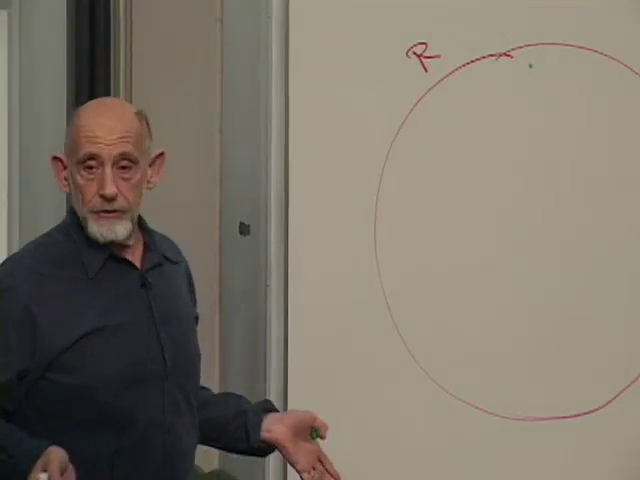
\includegraphics[width=0.74\textwidth]{lecture_09_figure_02.png}
  \caption{Phép tính đối chứng cho hạt điểm:
  \(p^2/(2m)=L^2/(2mR^2)=L^2/(2I)\).}
  \lectureframe{00:11:25}
  \label{fig:l09-sphere-rotor}
\end{figure}

Ví dụ không hề rắc rối này rất quan trọng. Bản thân độ cong không phải là vấn đề. Vấn đề xuất hiện khi độ cong ghép với độ trải rộng lượng tử nội tại của dây.

\section{Dây chân không không có dạng điểm}

Xét một tọa độ ngang của một dây mở và trừ đi tọa độ khối tâm của nó. Khai triển theo dao động tử dùng ở đây chỉ có tính sơ đồ:
\begin{equation}
  X(\sigma)-X_{\mathrm{cm}}
  \sim
  \sum_{n=1}^{\infty}
  \frac{a_n+a_n^\dagger}{\sqrt n}\cos(n\sigma).
  \label{eq:l09-mode-expansion}
\end{equation}
Các thành phần cốt yếu là các mode cosin, các toán tử dao động tử và thừa số \(1/\sqrt n\). Các chuẩn hóa chính xác không đóng vai trò nào trong lập luận về kích thước.
\editorialnote{Khai triển chính xác chứa các thừa số của \(\alpha'\) phụ thuộc vào quy ước, các hằng số số học và một lựa chọn ký hiệu dao động tử. Phương trình \eqref{eq:l09-mode-expansion} chỉ giữ lại sự phụ thuộc cần thiết cho ước lượng tử ngoại, đúng như trong phép suy dẫn trên bảng.}

\begin{figure}[H]
  \centering
  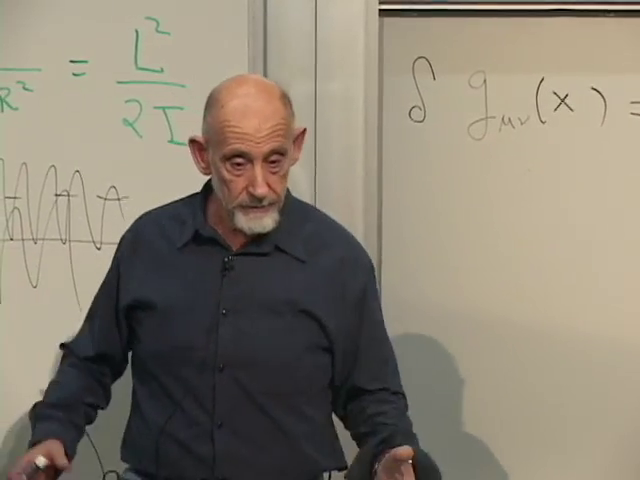
\includegraphics[width=0.78\textwidth]{lecture_09_figure_03.png}
  \caption{Khai triển dao động tử về mặt cấu trúc và tổng kép thu được khi bình phương nó.}
  \lectureframe{00:15:20}
  \label{fig:l09-string-modes}
\end{figure}

Bình phương khoảng cách tới khối tâm trong chân không của các dao động tử là
\begin{align}
  \expect{\bigl(X(\sigma)-X_{\mathrm{cm}}\bigr)^2}_0
  &\sim
  \sum_{n,m\geq1}
  \frac{\cos(n\sigma)\cos(m\sigma)}{\sqrt{nm}}\notag\\
  &\qquad\times
  \bra{0}(a_n+a_n^\dagger)\notag\\
  &\hspace{6em}\times(a_m+a_m^\dagger)\ket{0}.
  \label{eq:l09-size-double-sum}
\end{align}
Phần lớn các hạng đều triệt tiêu. Hai toán tử hủy triệt tiêu ket; hai toán tử tạo để lại một trạng thái trực giao với bra; và một toán tử tạo theo sau bởi một toán tử hủy cũng có giá trị kỳ vọng chân không bằng 0 trong thứ tự này. Phép co còn lại là
\begin{equation}
  \bra{0}a_n a_m^\dagger\ket{0}=\delta_{nm}.
  \label{eq:l09-vacuum-contraction}
\end{equation}

\begin{figure}[H]
  \centering
  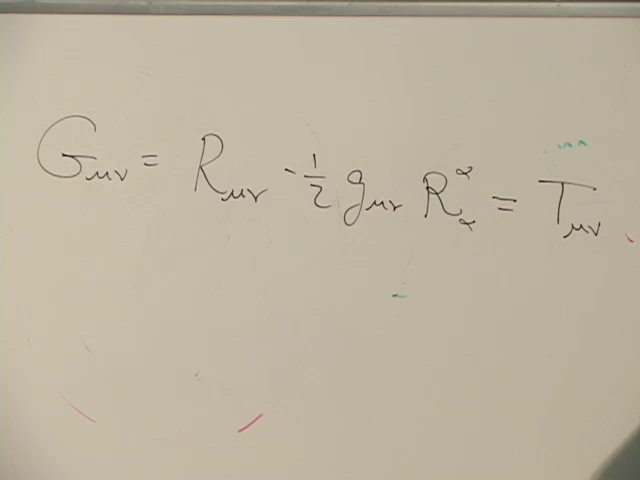
\includegraphics[width=0.74\textwidth]{lecture_09_figure_04.png}
  \caption{Phép co chân không còn lại rút tổng dao động tử kép về một tổng đơn.}
  \lectureframe{00:20:10}
  \label{fig:l09-vacuum-contraction}
\end{figure}

Do đó
\begin{equation}
  \expect{\bigl(X(\sigma)-X_{\mathrm{cm}}\bigr)^2}_0
  \sim
  \sum_{n=1}^{\infty}\frac{\cos^2(n\sigma)}{n}.
  \label{eq:l09-size-single-sum}
\end{equation}
Tại một điểm điển hình dọc theo dây, hoặc sau khi lấy trung bình theo \(\sigma\), \(\cos^2(n\sigma)\) đóng góp xấp xỉ \(1/2\). Với một ngưỡng cắt mode \(N\),
\begin{equation}
  \expect{\bigl(X-X_{\mathrm{cm}}\bigr)^2}_{0,N}
  \sim
  \frac{1}{2}\sum_{n=1}^{N}\frac{1}{n}
  =\frac{1}{2}\log N+O(1).
  \label{eq:l09-logarithmic-size}
\end{equation}

\begin{figure}[H]
  \centering
  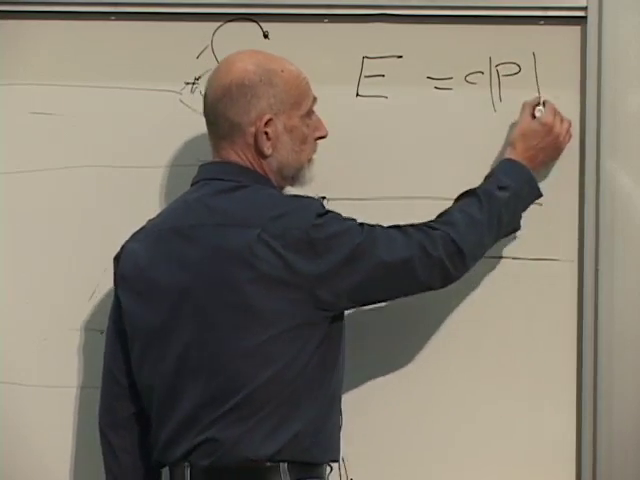
\includegraphics[width=0.72\textwidth]{lecture_09_figure_05.png}
  \caption{Trên bảng, ta đi đến tổng điều hòa chi phối độ trải rộng của trạng thái cơ bản.}
  \lectureframe{00:22:05}
  \label{fig:l09-harmonic-size}
\end{figure}

Chẳng hạn, nếu chỉ giữ 25 mode đầu tiên thì ta được một đối tượng mờ nhòe hữu hạn, nhưng đó vẫn chưa phải là dây trong giới hạn liên tục. Bỏ ngưỡng cắt đi làm cho độ trải rộng bình phương trung bình tăng theo logarit. Không nên hiểu nhầm kết luận này như một chứng minh rằng lý thuyết dây trong không gian phẳng là không nhất quán. Trong không gian phẳng, chuyển động của khối tâm và của các dao động tử tách rời nhau, và những sự triệt tiêu tinh tế trong các biên độ vật lý duy trì tính địa phương như kỳ vọng. Kích thước tăng dần là một lời cảnh báo. Độ cong cho ta biết liệu lời cảnh báo ấy có trở thành một thất bại hay không.

\section{Khi độ trải rộng nội tại làm thay đổi hình học}

Đặt dây gần cực bắc của mặt cầu. Khi mọi dao động tử đều bị tắt, nó ứng xử như hạt điểm vừa khảo sát. Khi cho phép các mode cao hơn, dây trở thành một bó rối dao động trải trên chỏm cầu. Khối tâm của nó vẫn có thể đi quanh mặt cầu, nhưng đối tượng có mômen quán tính đi vào năng lượng quay nay là một đối tượng mở rộng.

Đối với một trục đi qua tâm mặt cầu và các cực,
\begin{equation}
  I=\int r_\perp^2\,dm,
  \label{eq:l09-extended-inertia}
\end{equation}
trong đó \(r_\perp\) là khoảng cách vuông góc từ một phần tử dây tới trục ấy. Một điểm ở xích đạo của quỹ đạo có cánh tay đòn liên quan lớn nhất. Những phần của dây võng về phía trục đóng góp ít hơn. Với tổng khối lượng cố định, điều này làm giảm mômen quán tính hiệu dụng:
\begin{equation}
  I_{\mathrm{eff}}<mR^2.
  \label{eq:l09-inertia-reduction}
\end{equation}
Vì thế năng lượng quay có dạng như của một vật điểm trên một mặt cầu nhỏ hơn,
\begin{equation}
  E_{\mathrm{rot}}
  =\frac{L^2}{2I_{\mathrm{eff}}}
  \equiv \frac{L^2}{2mR_{\mathrm{eff}}^2},
  \qquad R_{\mathrm{eff}}<R.
  \label{eq:l09-effective-radius}
\end{equation}

\begin{classroomqa}
\audiencequestion{Vì sao mômen quán tính lại phải tiến về 0 nếu dây đang trải ra trên một vùng lớn hơn? \lecturetimestamp{00:33:23}}
\lecturerresponse{Phát biểu này nói về mô tả hiệu dụng dưới phép thô hóa liên tiếp, chứ không khẳng định rằng phân bố mở rộng ban đầu lập tức có mômen quán tính bằng 0. Dải mode đầu tiên biến điểm thành một khối mờ chuyển động như thể nó sống trên một mặt cầu nhỏ hơn. Dải kế tiếp phân giải cấu trúc bên trong mỗi khối như vậy và lặp lại đúng sự tái chuẩn hóa đó. Lặp lại phép so sánh ấy sẽ đẩy bán kính hiệu dụng vào phía trong.}
\end{classroomqa}

\begin{figure}[H]
  \centering
  \includegraphics[width=0.72\textwidth]{lecture_09_figure_06.png}
  \medskip

  \begin{adjustbox}{max width=\linewidth}
  \begin{tikzpicture}[x=1cm,y=1cm,>=Latex]
    \draw[thick] (0,0) circle (2.15);
    \draw[dashed] (0,-2.55) -- (0,2.55);
    \draw[blue!65!black,thick]
      (-0.22,2.05)
      .. controls (-1.22,1.75) and (-1.52,1.08) .. (-1.06,0.44)
      .. controls (-0.55,-0.10) and (0.35,0.02) .. (1.10,0.68)
      .. controls (1.48,1.12) and (1.16,1.80) .. (0.20,2.05);
    \draw[red!70!black,dashed] (0,0) circle (1.25);
    \draw[->] (2.70,1.55) -- (4.05,1.55);
    \node[align=center] at (3.37,1.98) {add shorter\\modes};
    \draw[thick] (6.15,0) circle (1.25);
    \draw[dashed] (6.15,-1.65) -- (6.15,1.65);
    \draw[blue!65!black,thick]
      (6.00,1.18)
      .. controls (5.42,0.88) and (5.46,0.25) .. (6.02,-0.06)
      .. controls (6.46,-0.28) and (6.90,0.45) .. (6.28,1.18);
    \node at (0,-3.00) {sphere of radius \(R\)};
    \node at (6.15,-2.05) {effective radius \(R_{\mathrm{eff}}\)};
  \end{tikzpicture}
  \end{adjustbox}
  \caption{Dây ở cực bắc trên bảng và một tái dựng gọn gàng của lập luận về bán kính hiệu dụng. Đường tròn đứt nét phía trong là một hình học hiệu dụng, không phải một vỏ vật lý thứ hai bên trong mặt cầu.}
  \lectureframe{00:35:15}
  \label{fig:l09-shrinking-sphere}
\end{figure}

Đây là một phát biểu của nhóm tái chuẩn hóa. Một ngưỡng cắt hữu hạn làm cho dây trở thành một khối với độ phân giải nội tại hữu hạn. Tăng ngưỡng cắt sẽ làm thay đổi cơ học của khối đó. Trên một mặt cầu có độ cong dương, mỗi lớp mode được thêm vào làm cho nền được suy ra từ chuyển động ở khoảng cách lớn trở nên nhỏ hơn. Nếu kết quả không bao giờ ổn định, thì không tồn tại một lý thuyết dây độc lập với ngưỡng cắt trên nền đó.

\section{Metric phải đạt tới một điểm bất động}

Bây giờ thay mặt cầu bằng một metric không gian đích tổng quát \(g_{\mu\nu}(x)\). Việc đưa thêm vào một lớp logarit mỏng các mode dao động tử làm thay đổi metric ấy bởi một tensor địa phương đối xứng hạng hai. Sự thay đổi đó phải triệt tiêu trong không gian phẳng và bắt đầu bằng hai đạo hàm của metric. Ở bậc dẫn đầu, tính hiệp biến để lại tensor Ricci như ứng viên thích hợp:
\begin{equation}
  \frac{\partial g_{\mu\nu}}{\partial\log\Lambda}
  =-C\,R_{\mu\nu}+\cdots ,
  \qquad C>0
  \label{eq:l09-ricci-flow}
\end{equation}
theo chiều thô hóa được dùng trong lập luận hình học. Khi đó độ cong dương đẩy mặt cầu vào trong, đúng như cần phải vậy.
\editorialnote{Chuẩn hóa và dấu phụ thuộc vào việc tham số tái chuẩn hóa tăng về phía tử ngoại hay về phía hồng ngoại. Trong ký hiệu mặt thế giới thông dụng, hàm beta của metric ở bậc dẫn đầu là \(\beta^g_{\mu\nu}=\alpha'R_{\mu\nu}+\cdots\). Phát biểu bất biến được dùng ở đây là tính độc lập với ngưỡng cắt đòi hỏi hàm beta, và do đó \(R_{\mu\nu}\) ở bậc này, phải triệt tiêu.}

\begin{figure}[H]
  \centering
  \includegraphics[width=0.76\textwidth]{lecture_09_figure_07.png}
  \caption{Sự biến đổi của metric được viết một cách sơ đồ là âm tensor Ricci, với một đường cong làm trơn được vẽ bên cạnh.}
  \lectureframe{00:43:00}
  \label{fig:l09-ricci-flow-board}
\end{figure}

\begin{classroomqa}
\audiencequestion{Ngưỡng cắt dao động tử \(N\) xuất hiện ở đâu trong phương trình dòng chảy này? \lecturetimestamp{00:43:38}}
\lecturerresponse{Nó chính là biến tỉ lệ. Tổng kích thước của dây thay đổi theo logarit khi mode cao nhất được đưa vào thay đổi, nên tham số tiến hóa tự nhiên là \(\log N\), hay tương đương \(\log\Lambda\). Phương trình \eqref{eq:l09-ricci-flow} mô tả biến thiên vi phân do một lớp logarit các mode gây ra.}
\end{classroomqa}

Một nền được chấp nhận là một điểm bất động của dòng chảy này. Ở bậc dẫn đầu,
\begin{equation}
  \boxed{R_{\mu\nu}=0.}
  \label{eq:l09-ricci-flat}
\end{equation}
Phẳng Ricci không có nghĩa là mọi thành phần của tensor Riemann đều triệt tiêu. Chẳng hạn, sóng hấp dẫn có thể có độ cong khác không trong chân không mà vẫn thỏa mãn \(R_{\mu\nu}=0\).

\subsection{Cùng điều kiện đó chính là phương trình Einstein chân không}

Bỏ qua các hằng số quy ước, phương trình Einstein là
\begin{equation}
  G_{\mu\nu}
  \equiv
  R_{\mu\nu}-\frac12 g_{\mu\nu}R
  =T_{\mu\nu}.
  \label{eq:l09-einstein}
\end{equation}

\begin{figure}[H]
  \centering
  \includegraphics[width=0.78\textwidth]{lecture_09_figure_08.png}
  \caption{Tensor Einstein và tensor ứng suất-năng lượng trên bảng.}
  \lectureframe{00:47:15}
  \label{fig:l09-einstein-board}
\end{figure}

Trong chân không \(T_{\mu\nu}=0\). Lấy vết trong không-thời gian \(D\) chiều cho
\begin{equation}
  0=g^{\mu\nu}G_{\mu\nu}
   =\left(1-\frac{D}{2}\right)R.
  \label{eq:l09-einstein-trace}
\end{equation}
Với \(D\neq2\) thì \(R=0\), và thế trở lại vào \eqref{eq:l09-einstein} thu được \(R_{\mu\nu}=0\). Vì vậy, điều kiện để dây mất sự phụ thuộc vào ngưỡng cắt chính là phương trình trường hấp dẫn chân không. Hấp dẫn không phải được gắn thêm vào lý thuyết; nó xuất hiện như cái giá phải trả cho tính nhất quán.

Từ \emph{chân không} không có nghĩa là không có gì xảy ra. Nó có nghĩa là trong vùng đó không có nguồn ứng suất-năng lượng. Các phương trình Maxwell không nguồn cho phép sóng điện từ, và các phương trình Einstein không nguồn cho phép sóng hấp dẫn. Hình học có thể vẫn là động ngay cả khi tensor Ricci của nó triệt tiêu.

\begin{classroomqa}
\audiencequestion{Điều kiện này có liên hệ với bất biến bảo giác không?
\lecturetimestamp{00:52:20}}
\lecturerresponse{Có, mặc dù câu hỏi trong bản ghi đã bị mất đi một phần. Đối xứng liên quan là bất biến bảo giác của lý thuyết lượng tử \emph{mặt thế giới}. Việc đòi hỏi dị thường tỉ lệ của mặt thế giới triệt tiêu chính là điều đặt hàm beta của metric bằng 0. Không nên nhầm điều đó với việc đòi hỏi bất biến bảo giác của bản thân không-thời gian.}
\end{classroomqa}

Còn có một điều kiện nhất quán thứ hai. Bất biến bảo giác của mặt thế giới cũng ấn định số chiều không-thời gian tới hạn: 10 đối với siêu dây và 26 đối với dây boson. Vì vậy, chỉ riêng tính phẳng Ricci chưa phải là danh sách đầy đủ các yêu cầu, nhưng đó là phần bộc lộ phương trình Einstein trực tiếp nhất.

\section{Các chiều compact chứ không phải các chiều bị thiếu}

Một phông nền siêu dây có 9 chiều không gian và 1 chiều thời gian. Thế giới vĩ mô của chúng ta chỉ biểu lộ 3 phương không gian lớn, nên 6 chiều không gian phải bị che giấu hoặc bằng cách khác trở nên không thể tiếp cận ở các thang đo thông thường. Sự compact hóa giữ chúng như những phương thực sự đồng thời cho chúng một kích thước hữu hạn nhỏ.

\begin{classroomqa}
\audiencequestion{Nếu các quan sát viên khác nhau mang theo những đồng hồ khác nhau, điều đó có đồng nghĩa với việc có nhiều hơn một chiều thời gian không? \lecturetimestamp{00:56:59}}
\lecturerresponse{Không. Nhiều đồng hồ là nhiều dụng cụ đo các tọa độ trong cùng một không-thời gian; chúng không tạo ra các phương thời gian độc lập. Các chiều phụ được xét ở đây là các chiều không gian. Các cấu trúc lượng tử và nhân quả quen thuộc không cung cấp một lý thuyết nhất quán tương đương với nhiều phương thời gian địa phương, nên khả năng đó không thuộc mô hình compact hóa này.}
\end{classroomqa}

Hãy tưởng tượng những sinh vật tin rằng thế giới của chúng là một đường thẳng. Ở độ phân giải thấp, chúng chỉ có thể di chuyển tới và lui. Tuy nhiên, dưới một kính hiển vi đủ mạnh, đường thẳng ấy lộ ra là một hình trụ rất mảnh. Một sinh vật nhỏ còn có thể di chuyển quanh phương tròn của nó cũng như dọc theo chiều dài của nó. Phương thứ hai ấy luôn hiện diện; chu vi của nó quá nhỏ để các đầu dò thô phân giải được.

\begin{figure}[H]
\centering
  \includegraphics[width=0.78\textwidth]{lecture_09_figure_09.png}
\caption{Một hình trụ hẹp và các quỹ đạo quấn quanh phương tròn ẩn của nó.}
\lectureframe{01:01:00}
\label{fig:l09-hidden-cylinder}
\end{figure}

Một hình trụ có thể được biểu diễn như một dải mà cạnh trên và cạnh dưới được đồng nhất với nhau. Đi qua cạnh trên thì sẽ trở lại qua cạnh dưới tại cùng một vị trí dọc theo chiều dài. Không có biên vật lý ở cạnh nào cả. Có thể thực hiện thao tác tương tự với hai phương: đồng nhất cạnh trái và cạnh phải của một hình chữ nhật, đồng thời cả cạnh trên và cạnh dưới của nó. Kết quả là một xuyến hai chiều.

\begin{figure}[H]
  \centering
  \includegraphics[width=0.76\textwidth]{lecture_09_figure_10.png}
  \medskip

\begin{tikzpicture}[x=0.82cm,y=0.82cm,>=Latex]
    \draw[thick] (0,0) rectangle (4,2.15);
    \draw[blue!65!black,->] (0,2.48) -- (4,2.48);
    \draw[blue!65!black,->] (4,-0.34) -- (0,-0.34);
    \node at (2,-0.82) {one periodic direction};
    \draw[thick] (6.1,0) rectangle (10.1,2.15);
    \draw[blue!65!black,->] (6.1,2.48) -- (10.1,2.48);
    \draw[blue!65!black,->] (10.1,-0.34) -- (6.1,-0.34);
    \draw[red!70!black,->] (5.76,0) -- (5.76,2.15);
    \draw[red!70!black,->] (10.44,2.15) -- (10.44,0);
    \node at (8.1,-0.82) {two periodic directions};
  \end{tikzpicture}
\caption{Tấm phiến trên bảng và một mô tả rõ ràng bằng miền cơ bản. Đồng nhất một cặp cạnh cho ta một hình trụ; đồng nhất cả hai cặp cho ta một xuyến.}
\lectureframe{01:04:40}
\label{fig:l09-periodic-identification}
\end{figure}

Xuyến trước hết là một tôpô học, trước khi là một mặt có dạng bánh vòng trong không gian ba chiều. Cắt một xuyến một lần thì nó trở thành một hình trụ; cắt thêm một lần nữa thì nó trở thành một hình chữ nhật, miễn là vẫn ghi nhớ các phép đồng nhất cạnh. Có thể đặt một metric phẳng lên hình chữ nhật này, nên xuyến phẳng thu được có độ cong Riemann bằng không cục bộ và chắc chắn là Ricci-phẳng.

Một quỹ đạo thẳng trên hình chữ nhật tiếp tục đi thẳng qua một cạnh được đồng nhất. Nếu hệ số góc của nó là một tỉ số hữu tỉ của hai chu kỳ, quỹ đạo cuối cùng sẽ khép kín. Nếu tỉ số ấy là vô tỉ, nó không bao giờ khép kín và trở nên trù mật trên xuyến.

\begin{figure}[H]
\centering
  \includegraphics[width=0.76\textwidth]{lecture_09_figure_11.png}
\caption{Các đoạn thẳng lặp lại trong một miền cơ bản biểu diễn một quỹ đạo liên tục không đứt đoạn duy nhất trên xuyến.}
\lectureframe{01:11:00}
\label{fig:l09-torus-trajectory}
\end{figure}

Các xuyến nhiều chiều hơn được tạo thành theo đúng cách ấy. Một hình lập phương mà mỗi cặp mặt đối diện được đồng nhất là một xuyến ba chiều, và 6 phương compact có thể được mô hình hóa bằng một xuyến sáu chiều. Không nên cố nhúng tất cả các đối tượng này vào không gian ba chiều thông thường; mô tả bằng phép đồng nhất các mặt là nội tại và đầy đủ.

\begin{classroomqa}
\audiencequestion{Một chiều phụ có nhất thiết phải tự khép lại không?
\lecturetimestamp{01:15:03}}
\lecturerresponse{Không như một định lý. Nó có thể không compact, nhưng khi đó bình thường nó sẽ xuất hiện như một phương lớn khác trong thế giới khoảng cách xa mà ta quan sát được. Tính compact là cách đơn giản nhất để dung hòa các chiều phụ với sự vắng mặt bề ngoài của chúng. Vì sao tự nhiên chọn một compact hóa cụ thể là một câu hỏi động lực học riêng.}
\end{classroomqa}

\begin{classroomqa}
\audiencequestion{Vì sao lại giả sử các chiều không nhìn thấy là những phương không gian thông thường cuộn lại theo cách này, thay vì một cái gì hoàn toàn khác? \lecturetimestamp{01:15:51}}
\lecturerresponse{Bởi vì đây là một giả thuyết xác định có thể giải được, chứ không phải vì nó đã được chứng minh là mô tả duy nhất của tự nhiên. Các đa tạp không gian compact cho phép ta xây dựng những ví dụ nhất quán và tính phổ của chúng. Những khả năng kỳ lạ hơn phải giành được chỗ đứng của mình bằng cách làm được điều tương tự.}
\end{classroomqa}

\begin{classroomqa}
\audiencequestion{Các khoảng cách trên xuyến quen thuộc có dạng bánh vòng không giống các khoảng cách trong một hình chữ nhật. Ở đây hiểu hình học nào?
\lecturetimestamp{01:18:11}}
\lecturerresponse{Thuật ngữ \emph{xuyến} cố định các phép đồng nhất, chứ không cố định một metric duy nhất. Hình bánh vòng được nhúng thừa hưởng một metric cong từ không gian ba chiều. Hình chữ nhật được đồng nhất tuần hoàn mang một metric phẳng. Chúng có cùng tôpô nhưng hình học khác nhau; đối với compact hóa đơn giản, điều chúng ta muốn nói là loại phẳng.}
\end{classroomqa}

\section{Các tham số hình dạng của một xuyến phẳng}

Ngay cả một xuyến phẳng hai chiều cũng không là duy nhất. Hình bình hành cơ bản của nó có một diện tích tổng thể, một tỉ số cạnh, và một độ xiên. Thay đổi các tham số này làm thay đổi các khoảng cách và vì thế làm thay đổi phổ, mà không làm thay đổi tôpô.

\begin{figure}[H]
  \centering
  \includegraphics[width=0.74\textwidth]{lecture_09_figure_12.png}
  \medskip

\begin{tikzpicture}[x=0.9cm,y=0.9cm,>=Latex]
    \draw[thick] (0,0) rectangle (3.4,2.1);
    \draw[<->] (0,-0.35) -- node[below] {\(L_1\)} (3.4,-0.35);
    \draw[<->] (-0.35,0) -- node[left] {\(L_2\)} (-0.35,2.1);
    \draw[thick] (5.4,0) -- (8.8,0) -- (9.7,2.1) -- (6.3,2.1) -- cycle;
    \draw[dashed] (5.4,0) -- (6.3,2.1);
    \draw[->] (5.75,2.48) -- node[above] {shear} (6.45,2.48);
    \node at (1.7,-1.00) {area and aspect ratio};
    \node at (7.55,-1.00) {complex structure};
  \end{tikzpicture}
\caption{Các miền cơ bản hình chữ nhật và hình xiên dùng để thảo luận các môđun của xuyến.}
\lectureframe{01:23:00}
\label{fig:l09-torus-moduli}
\end{figure}

Đối với một xuyến hai chiều, thật tiện khi mã hóa hình dạng của nó bằng một số phức \(\tau=\tau_1+i\tau_2\): phần thực ghi lại độ xiên và phần ảo ghi lại tỉ số cạnh sau khi đã tách riêng thang tỉ lệ tổng thể. Hoán đổi hai chu trình cơ bản hoặc thay đổi cơ sở nguyên của chúng có thể khiến những hình bình hành bề ngoài khác nhau mô tả cùng một xuyến.

\begin{classroomqa}
\audiencequestion{Điều gì xảy ra nếu một cạnh bị lật trước khi đồng nhất? \lecturetimestamp{01:24:20}}
\lecturerresponse{Khi đó tạo ra một tôpô khác. Đồng nhất kèm theo một phép phản xạ cho một mặt không định hướng, chai Klein, chứ không phải một xuyến thông thường.}
\end{classroomqa}

\begin{classroomqa}
\audiencequestion{Nếu độ xoắn không đều dọc theo cạnh thì sao?
\lecturetimestamp{01:25:01}}
\lecturerresponse{Một biến dạng trơn không đều có thể được chuyển vào metric trên miền cơ bản. Phải giữ tách biệt phép đồng nhất tôpô và dữ liệu hình học: thay đổi cách dán có thể làm thay đổi tôpô, còn thay đổi trơn các khoảng cách thì làm thay đổi metric.}
\end{classroomqa}

\editorialnote{Đối với một xuyến phẳng hai chiều, diện tích là môđun Kahler đơn giản nhất và \(\tau\) là môđun cấu trúc phức. Một độ xiên liên tục là một phần của \(\tau\). Trái lại, một phép xoắn Dehn là một thao tác lớp ánh xạ rời rạc, được biểu diễn bởi \(\tau\mapsto\tau+1\); bản thân nó không phải là môđun liên tục. Điều này làm rõ hơn thuật ngữ cố ý không quá hình thức đã dùng trong phần thảo luận trên bảng.}

Các xuyến phẳng hữu ích vì chúng thỏa mãn ngay điều kiện nhất quán, nhưng đối xứng của chúng quá lớn đối với một mô hình vật lý hạt hiện thực. Những không gian Ricci-phẳng phức tạp hơn, đặc biệt là các đa tạp Calabi--Yau, cung cấp những compact hóa phong phú hơn. Cách xây dựng chi tiết của chúng vượt ra ngoài phần thảo luận này; nguyên lý vẫn như nhau.

\section{Suy ra một đường tròn compact từ phổ của nó}

Sau giờ nghỉ, ta thu gọn không gian compact còn một đường tròn có chu vi \(2\pi R\). Một hàm sóng phải đơn trị sau một vòng đi hết đường tròn:
\begin{equation}
  e^{ip_c(x+2\pi R)/\hbar}=e^{ip_cx/\hbar}.
\end{equation}
Do đó
\begin{equation}
  p_cR=n\hbar,
  \qquad
  p_c=\frac{n\hbar}{R},
  \qquad n\in\mathbb Z.
  \label{eq:l09-kk-momentum}
\end{equation}

\begin{figure}[H]
\centering
  \includegraphics[width=0.74\textwidth]{lecture_09_figure_13.png}
\caption{Chu vi compact \(2\pi R\) và xung lượng lượng tử hóa \(p_c=n\hbar/R\).}
\lectureframe{01:32:15}
\label{fig:l09-kk-board}
\end{figure}

Đối với một hạt không khối lượng trong toàn bộ không-thời gian,
\begin{equation}
  E=c|\mathbf P|.
  \label{eq:l09-massless-dispersion}
\end{equation}

\begin{figure}[H]
\centering
  \includegraphics[width=0.70\textwidth]{lecture_09_figure_14.png}
\caption{Hệ thức tán sắc không khối lượng được dùng để diễn giải lại xung lượng compact như khối lượng ở số chiều thấp hơn.}
\lectureframe{01:33:45}
\label{fig:l09-massless-board}
\end{figure}

Tách xung lượng thành phần không compact và phần compact, rồi đặt \(c=\hbar=1\):
\begin{equation}
  E^2=\mathbf p_{\mathrm{large}}^2+\frac{n^2}{R^2}.
  \label{eq:l09-kk-dispersion}
\end{equation}
Một quan sát viên không thể phân giải phương compact sẽ so sánh điều này với \(E^2=\mathbf p_{\mathrm{large}}^2+m^2\) và suy ra một tháp khối lượng
\begin{equation}
  m_n=\frac{|n|}{R}.
  \label{eq:l09-kk-masses}
\end{equation}
Hai dấu của \(n\) mô tả các xung lượng compact ngược chiều nhau với cùng năng lượng dương, chứ không phải các khối lượng dương và âm. Vì vậy, khoảng cách mức \(1/R\) cho phép suy ra bán kính bằng quang phổ. Đây là cơ chế Kaluza--Klein: xung lượng theo một phương ẩn xuất hiện như khối lượng trong các chiều nhìn thấy.

\section{Các trạng thái quấn hoàn thiện phổ}

Một dây kín có một khả năng mà hạt điểm không có: nó có thể quấn quanh đường tròn. Nếu số quấn là \(w\), dây chỉ khép kín sau khi đi hết phương compact \(w\) lần. Độ dài của nó là \(2\pi |w|R\), nên lực căng cung cấp một năng lượng
\begin{equation}
  m_w
  =2\pi T\,|w|R
  =\frac{|w|R}{\alpha'}.
  \label{eq:l09-winding-mass}
\end{equation}
Bài giảng chọn các đơn vị sao cho \(\alpha'=1\), nhờ đó biểu thức này rút gọn thành
\begin{equation}
  m_w=|w|R.
  \label{eq:l09-winding-lecture-units}
\end{equation}
Các giá trị dương và âm của \(w\) tương ứng với hai hướng ngược nhau quanh đường tròn.

\begin{figure}[H]
\centering
  \includegraphics[width=0.76\textwidth]{lecture_09_figure_15.png}
\caption{Một dây kín quấn quanh hình trụ compact, với bán kính compact được đánh dấu trên bảng.}
\lectureframe{01:39:45}
\label{fig:l09-winding-board}
\end{figure}

Vì vậy, đường tròn compact tạo ra hai dãy mức bổ sung cho nhau:
\begin{equation}
  m_n=\frac{|n|}{R},
  \qquad
  m_w=\frac{|w|R}{\alpha'}.
  \label{eq:l09-two-towers}
\end{equation}
Khi \(R\) lớn, các mức xung lượng sít nhau và các trạng thái quấn nặng. Khi \(R\) nhỏ, các mức xung lượng cách xa nhau và các trạng thái quấn nhẹ.

\begin{figure}[H]
\centering
  \begin{tikzpicture}[x=1cm,y=0.9cm,>=Latex]
    \draw[->] (0,0) -- (0,4.7) node[above] {\(m\)};
    \foreach \y/\lab in {0/0,1.1/{1/R},2.2/{2/R},3.3/{3/R},4.4/{4/R}} {
      \draw (-0.16,\y) -- (0.16,\y);
      \node[left] at (-0.22,\y) {\(\lab\)};
    }
    \node at (0,-0.62) {momentum};
    \draw[<->,very thick,blue!65!black] (2.05,2.15) -- (4.05,2.15)
      node[midway,above] {\(R\leftrightarrow\alpha'/R\)};
    \draw[->] (6.1,0) -- (6.1,4.7) node[above] {\(m\)};
    \foreach \y/\lab in {0/0,1.1/{R/\alpha'},2.2/{2R/\alpha'},3.3/{3R/\alpha'},4.4/{4R/\alpha'}} {
      \draw (5.94,\y) -- (6.26,\y);
      \node[right] at (6.32,\y) {\(\lab\)};
    }
    \node at (6.1,-0.62) {winding};
  \end{tikzpicture}
\caption{Các tháp xung lượng và quấn hoán đổi cho nhau khi bán kính được đảo nghịch trong đơn vị dây.}
\label{fig:l09-dual-mass-towers}
\end{figure}

\section{Đối ngẫu T: đường tròn nhỏ và lớn cho cùng một vật lý}

Hai tháp hoán đổi cho nhau dưới phép
\begin{equation}
  R\longleftrightarrow\frac{\alpha'}{R},
  \qquad
  n\longleftrightarrow w.
  \label{eq:l09-t-duality}
\end{equation}
Trong các đơn vị dùng trên bảng, \(\alpha'=1\), nên điều này đơn giản là
\(R\leftrightarrow1/R\). Ở bán kính tự đối ngẫu
\(R=\sqrt{\alpha'}\), các thang xung lượng và quấn trùng nhau.

\begin{figure}[H]
\centering
  \includegraphics[width=0.74\textwidth]{lecture_09_figure_16.png}
\caption{Các dãy khối lượng thưa và dày được so sánh trên bảng khi bán kính đi qua thang tự đối ngẫu.}
\lectureframe{01:43:00}
\label{fig:l09-duality-board}
\end{figure}

Việc hoán đổi các công thức khối lượng sơ cấp chỉ là phần bề mặt dễ thấy của kết quả. Các trạng thái dao động của dây kín và các biên độ tán xạ cũng được ánh xạ một cách nhất quán. Một đường tròn nhỏ hơn thang dây không phải là một hình học mới ngày càng tí hon; nó có một mô tả tương đương như một đường tròn đối ngẫu lớn hơn. Hạt điểm không thể thực hiện sự đồng nhất này vì chúng có các mode xung lượng nhưng không có các mode quấn.

\begin{classroomqa}
\audiencequestion{Điều này có đơn thuần chỉ là hoán đổi một phương thẳng đứng với một phương nằm ngang không? \lecturetimestamp{01:44:38}}
\lecturerresponse{Không. Nó hoán đổi hai số lượng tử khác nhau: xung lượng quanh đường tròn và số lần một dây kín quấn quanh đường tròn. Đồng thời bán kính cũng phải bị đảo nghịch.}
\end{classroomqa}

\begin{classroomqa}
\audiencequestion{Các mô tả tại \(R<\sqrt{\alpha'}\) và \(R>\sqrt{\alpha'}\) chỉ nói về boson, hay cũng áp dụng cho fermion?
\lecturetimestamp{01:46:30}}
\lecturerresponse{Đối ngẫu là một đối xứng của toàn bộ lý thuyết dây compact hóa, chứ không chỉ của tháp khối lượng boson đơn giản dùng để làm lộ ra nó. Ánh xạ chi tiết giữa các sector phụ thuộc vào lý thuyết, nhưng sự tương đương nhỏ--lớn không bị giới hạn ở một loài hạt duy nhất.}
\end{classroomqa}

\begin{classroomqa}
\audiencequestion{Hai trạng thái được so sánh là dây mở hay dây kín? \lecturetimestamp{01:47:32}}
\lecturerresponse{Chúng là các trạng thái dây kín. Một dây kín lan truyền tự do có thể quấn một đường tròn compact. Một dây mở thông thường với các đầu mút tự do không mang cùng số quấn bảo toàn ấy.}
\end{classroomqa}
\editorialnote{Trong trình bày đầy đủ hơn về dây mở, đối ngẫu T hoán đổi các điều kiện biên Neumann và Dirichlet và đưa vào các D-brane. Đó là lý do vì sao đối ngẫu T của dây mở phong phú hơn việc đơn giản sao chép công thức quấn của dây kín.}

\begin{classroomqa}
\audiencequestion{Sự hoán đổi này có tương tự như sự hoán đổi giữa không gian và thời gian gần chân trời lỗ đen không? \lecturetimestamp{01:48:00}}
\lecturerresponse{Không. Các tọa độ chân trời và tính chất nhân quả là một vấn đề khác. Ở đây hai mô tả liên quan đến một đường tròn không gian compact duy nhất và sự hoán đổi giữa các sector xung lượng và quấn của nó.}
\end{classroomqa}

\begin{classroomqa}
\audiencequestion{Điều này có chữa được vấn đề tự năng ở khoảng cách ngắn bằng cách đưa vào một độ dài tối thiểu không? \lecturetimestamp{01:48:35}}
\lecturerresponse{Nó cho thấy rằng các bán kính nhỏ hơn thang dây không xác định những nền đường tròn mới không tương đương: giảm \(R\) xuống dưới điểm tự đối ngẫu thì làm tăng bán kính đối ngẫu. Đây là một sự cản trở kiểu lý thuyết dây chính xác đối với việc thăm dò hình học đường tròn nhỏ tùy ý, mặc dù không nên biến điều đó thành khẳng định rằng mọi khái niệm khoảng cách có thể hình dung đều có một cận dưới cứng phổ quát duy nhất.}
\end{classroomqa}

\section{Vì sao không thể bỏ qua các sector quấn}

\begin{classroomqa}
\audiencequestion{Liệu ta có thể định nghĩa lý thuyết chỉ bằng các dây không quấn và bỏ các trạng thái quấn ra ngoài không? \lecturetimestamp{01:48:56}}
\lecturerresponse{Không. Các tương tác dây kín sinh ra chúng. Hãy kéo giãn một vòng không quấn quanh phương compact sao cho một đoạn đi theo đường tròn theo một chiều còn một đoạn khác đi theo chiều ngược lại. Tổng số quấn vẫn bằng không. Khi đó, một sự tái nối có thể tách vòng này thành hai dây kín có số quấn \(+1\) và \(-1\). Cặp đó có thể tách xa nhau, nên các trạng thái quấn phải thuộc về phổ ngay cả khi trạng thái ban đầu không có trạng thái nào như thế.}
\end{classroomqa}

\begin{figure}[H]
  \centering
  \includegraphics[width=0.74\textwidth]{lecture_09_figure_17.png}
  \caption{Vòng có số quấn bằng không được kéo giãn và bố trí quanh phương compact trước khi tái nối.}
  \lectureframe{01:50:30}
  \label{fig:l09-winding-pair-before}
\end{figure}

\begin{figure}[H]
  \centering
  \includegraphics[width=0.72\textwidth]{lecture_09_figure_18.png}
  \medskip

  \begin{tikzpicture}[x=0.9cm,y=0.9cm,>=Latex]
    \draw[thick] (0,0) ellipse (1.0 and 1.55);
    \draw[blue!65!black,thick]
      (0.08,1.35) .. controls (2.0,1.15) and (2.0,-1.15) .. (0.08,-1.35);
    \draw[red!70!black,thick]
      (-0.08,-1.35) .. controls (-2.0,-1.15) and (-2.0,1.15) .. (-0.08,1.35);
    \node at (0,-2.15) {net \(w=0\)};
    \draw[->,thick] (2.45,0) -- (3.75,0) node[midway,above] {split};
    \draw[thick] (5.05,0.62) ellipse (0.68 and 1.02);
    \draw[blue!65!black,very thick,->]
      (5.05,1.64) arc[start angle=90,end angle=-250,x radius=0.68,y radius=1.02];
    \node at (5.05,-0.82) {\(w=+1\)};
    \draw[thick] (7.45,0.62) ellipse (0.68 and 1.02);
    \draw[red!70!black,very thick,<-]
      (7.45,1.64) arc[start angle=90,end angle=-250,x radius=0.68,y radius=1.02];
    \node at (7.45,-0.82) {\(w=-1\)};
  \end{tikzpicture}
  \caption{Vòng quấn đã tách rời trên bảng và một cách dựng lại sáng sủa của quá trình tạo cặp quấn--phản quấn. Tổng số quấn vẫn bằng không.}
  \lectureframe{01:51:30}
  \label{fig:l09-winding-pair-after}
\end{figure}

\begin{classroomqa}
\audiencequestion{Việc tạo ra cặp quấn có đòi hỏi thêm năng lượng không?
\lecturetimestamp{01:52:11}}
\lecturerresponse{Có. Kéo giãn một dây tiêu tốn năng lượng do sức căng, và các dây quấn ở trạng thái cuối có các khối lượng như trong \eqref{eq:l09-winding-mass}. Một va chạm đủ năng lượng có thể tạo ra cặp đó, cũng như một va chạm có thể tạo ra một hạt và phản hạt của nó mà vẫn bảo toàn điện tích bảo toàn tương ứng.}
\end{classroomqa}

\section{Liệu ta có thể nghe ra hình dạng của một nền dây không?}

Đối với một lý thuyết hạt compact hóa thông thường, khoảng cách giữa các mức của phổ Kaluza--Klein cho phép ta suy ra bán kính: người ta cố nghe ra hình dạng của không gian compact từ các mode chuẩn của nó. Lý thuyết dây làm cho bài toán ngược này trở nên tinh tế hơn. Các mode xung lượng nghe \(1/R\), các mode quấn nghe \(R/\alpha'\), và toàn bộ phổ không đổi khi hoán đổi hai thứ đó. Hai bán kính mà hình học hạt điểm xem là khác nhau lại là một nền dây duy nhất được mô tả bằng các biến đối ngẫu.

Vì vậy, bài giảng bằng một con đường duy nhất đã đi tới cả hai kết luận đã hứa của nó. Tính nhất quán tử ngoại buộc metric đích phải thỏa mãn phương trình Einstein chân không, nên hấp dẫn là không thể tránh khỏi. Sau đó, sự compact hóa biến hình học ẩn thành các phổ hạt, nhưng các trạng thái quấn ngăn phổ đó gán một bán kính cổ điển duy nhất ở dưới thang dây. Tính nhất quán không chỉ lựa chọn những hình học nào được phép; thông qua đối ngẫu T, nó còn thay đổi ngay cả điều gì được tính là một hình học phân biệt.